\documentclass[a4paper]{article}
\usepackage[left=4cm, right=4cm, bottom=3.5cm, top=3.5cm]{geometry}
\usepackage{graphicx}

\usepackage[hyperfootnotes=false]{hyperref}
\usepackage{amsfonts, amsbsy, amssymb, amsmath}

\begin{document}

\def \cK {\mathcal{K}}

\section{Introduction}
\label{sec:intro}

This paper is outlined as follows: In Sec.\ \ref{sec:CMR} we introduce Chesnavich's Hamiltonian model  
for ion-molecule reaction and discuss the dynamical mechanism underlying roaming in 
terms of families of unstable periodic orbits and their associated invariant manifolds.

\section{Chesnavich's Model and Roaming}
\label{sec:CMR}
\subsection{Chesnavich's Model Hamiltonian}


The  CH$_4^+$ model due to Chesnavich  is a 2 degree of freedom Hamiltonian system  
comprised of a rigid CH$_3^+$ molecule (core) and a mobile H atom \cite{Chesnavich1986}. 
The system Hamiltonian is \cite{ezra2019chesnavich}
\begin{equation}
H(r,\theta,p_r, p_\theta) = \frac{1}{2} \frac{p_r^2}{\mu} + \frac{1}{2}p_\theta^2 \left(\frac{1}{\mu r^2}+\frac{1}{I_{CH_3}}\right) + U(r,\theta),
\label{eq:chesHam}
\end{equation}
where $(r, \theta, \phi)$ are polar coordinates describing the position of the 
H-atom in a body-fixed frame attached to the CH$_3^+$ core
(the coordinate $\phi$ is ignorable in this model).  
The reduced mass of the system is given by the expression 
$\mu=\frac{m_{CH_3}m_{H}}{m_{CH_3}+m_{H}}$, where $m_{H}=1.007825$ u and $m_{CH_3}=3m_{H}+12.0$ u, 
and the moment of inertia of the rigid body CH$_3^+$ has the value  $I_{CH_3}=2.373409$~u\AA$^2$.

The potential energy function $U(r,\theta)$ is made up  of a radial long range potential
energy term $U_{CH}$ and a short range potential $U_{coup}$ that models the short range anisotropy of the rigid CH$_3^+$ core:
\begin{equation}\label{eq:U}
 U(r,\theta ) = U_{CH} (r) + U_{coup} (r,\theta).
\end{equation}

The topography of the potential energy surface  is characterised by two deep wells that 
correspond to the  bound CH$_4^+$, two areas of high potential and a flat area to the outside 
of these features as shown in Fig. \ref{fig:pot}.

\begin{figure}[ht]
 \centering
 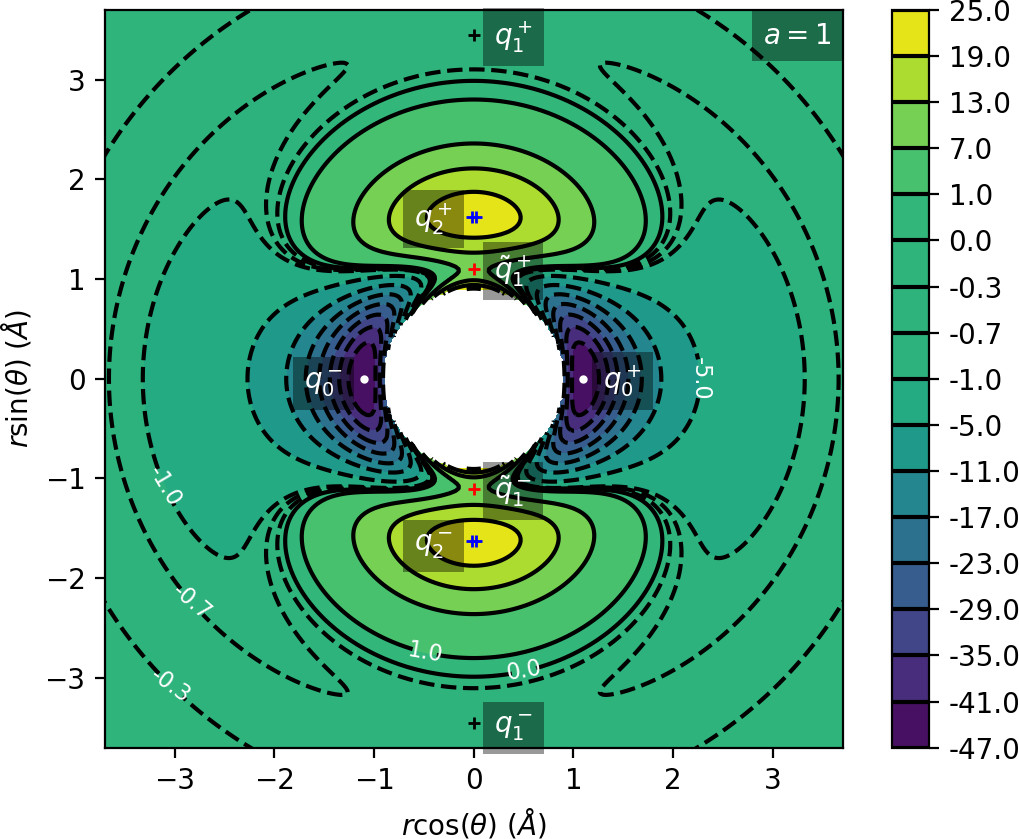
\includegraphics[width=.5\textwidth]{figure1}
 \caption{Contour plot of Chesnavich's potential energy surface $U$ for $a=1$. Dashed lines correspond to $U<0$, solid lines correspond to $U\geq0$. Contours correspond to values of potential shown on the colorbar to the right, with some values indicated in the plot. This figure is from \cite{krajnak2018influence}.
 }
 \label{fig:pot}
\end{figure}

The long range potential has the form:
\begin{equation}\label{eq:UCH}
 U_{CH} (r) =  \frac{D_e}{c_1 - 6} \left( 2 (3-c_2) e^{c_1 (1-x)}  - \left( 4 c_2 - c_1 c_2 + c_1 \right) x^{-6} - (c_1 - 6) c_2 x^{-4} \right), 
\end{equation}
where $x = \frac{r}{r_e}$ and we take the  parameter values as  in the original work \cite{Chesnavich1986}.
The short range hindered rotor  potential $U_{coup}$ has the form:
\begin{equation}\label{eq:Ucoup}
 U_{coup} (r,\theta) = \frac{U_e e^{-a(r-r_e)^2}}{2} (1 - \cos 2 \theta ),
\end{equation}
where $U_e$ is the equilibrium barrier height. 
The distance at which the  transition occurs from rotation to vibration is 
determined by the parameter $a$ (in \AA$^{-2}$). 
Various values of $a$ have been considered in previous works. In particular,  
$a=1$ \cite{Chesnavich1986,mauguiere2014roaming,mauguiere2014multiple,krajnak2018phase}, 
$a=4$ \cite{Chesnavich1986,mauguiere2014roaming} and a range of values $0.7\leq a\leq 8$. \cite{krajnak2018influence}

The CH$_3^+$ core is a symmetric top in Chesnavich's model. 
Although the range of the coordinate $\theta$ is $0 \leq \theta \leq \pi$, 
in the planar (zero overall angular momentum) version of the model the range of $\theta$ 
is extended to $0 \leq \theta \leq 2 \pi$, and the potential has a four-fold symmetry:
\begin{equation}
U(r,\theta)=U(r,-\theta)=U(r,\pi-\theta)=U(r,\pi+\theta).
\label{eq:sym}
\end{equation}

The potential admits four pairs of equilibrium points pairwise related by symmetry \eqref{eq:sym}, 
as listed in Tab. \ref{table:equil} and shown in Fig. \ref{fig:pot}.
  
  \begin{table}[ht]
    \begin{center}
    \begin{tabular}{c|c|c|c|c}
%     \hline\hline
    Energy (kcal mol$^{-1}$) & $r$ (\AA) & $\theta$ (radians) & Significance & Label \\
    \hline%\hline
    $-47$ & $1.1$ & $0$ & potential well & $q_0^+$ \\
    $-0.63$ & $3.45$ & $\pi/2$ & isomerisation saddle & $q_1^+$ \\
    $8$ & $1.1$ & $\pi/2$ & isomerisation saddle & $\widetilde{q}_1^+$ \\
    $22.27$ & $1.63$ & $\pi/2$ & local maximum & $q_2^+$ \\
%     \hline\hline
    \end{tabular}
    \end{center}
    \caption{Equilibrium points of the potential $U(r, \theta)$.}
    \label{table:equil}
   \end{table}

\bibliographystyle{plain}
\bibliography{allrefs}

\end{document}
